\documentclass{article}
\usepackage{amsmath}
\usepackage{amssymb}
\usepackage{geometry}
\usepackage{listings}
\usepackage{xcolor}
\usepackage{tikz}
\usepackage{booktabs}
\usetikzlibrary{arrows.meta, positioning, calc, shapes.geometric, fit, patterns}

\geometry{a4paper, margin=0.6in}

\definecolor{codegreen}{rgb}{0,0.6,0}
\definecolor{codepink}{rgb}{0.9,0.1,0.5}
\definecolor{codegray}{rgb}{0.5,0.5,0.5}
\definecolor{codepurple}{rgb}{0.58,0,0.82}
\definecolor{backcolour}{rgb}{0.97,0.97,0.97}

\lstdefinestyle{mystyle}{
    backgroundcolor=\color{backcolour},   
    commentstyle=\color{codegreen},
    keywordstyle=\color{blue},
    numberstyle=\tiny\color{codegray},
    stringstyle=\color{codepurple},
    basicstyle=\ttfamily\footnotesize,
    breakatwhitespace=false,         
    breaklines=true,                 
    captionpos=b,                    
    keepspaces=true,                 
    numbers=left,                    
    numbersep=5pt,                  
    showspaces=false,                
    showstringspaces=false,
    showtabs=false,                  
    tabsize=4
}
\lstset{style=mystyle}

\begin{document}

\title{\textbf{Mathematical Proofs, Shape Transitions, and Structural Flows of Low-Rank Adaptation (LoRA)}}
\author{Chief Strategist J}
\date{\today}
\maketitle

\section{Introduction and Intrinsic Dimension Hypothesis}
Fine-tuning a large causal language model like Qwen2.5-0.5B requires optimizing high-dimensional parameter spaces. For a linear layer parameter matrix $W_0 \in \mathbb{R}^{d \times k}$, full parameter updates can be represented as:
\begin{equation}
    W = W_0 + \Delta W
\end{equation}
Computing and storing updates $\Delta W$ directly requires maintaining optimizer states of size $O(d \cdot k)$ parameters per layer. Low-Rank Adaptation (LoRA) operates on the hypothesis that the update matrix $\Delta W$ resides in a subspace with a very low intrinsic dimension or rank $r \ll \min(d, k)$. Consequently, we define the update matrix by factorizing it:
\begin{equation}
    \Delta W = \frac{\alpha}{r} B A
\end{equation}
where $B \in \mathbb{R}^{d \times r}$ and $A \in \mathbb{R}^{r \times k}$ are trainable, while the original $W_0$ is frozen.

\section{Index-Level Derivation of Backpropagation}
Let $x \in \mathbb{R}^{1 \times d}$ be the row-vector input activation. The output projection $h \in \mathbb{R}^{1 \times k}$ is:
\begin{equation}
    h_j = \sum_{i=1}^d x_i (W_0)_{ij} + \frac{\alpha}{r} \sum_{p=1}^r \left( \sum_{i=1}^d x_i B_{ip} \right) A_{pj}
\end{equation}
Let $\mathcal{L}$ be the scalar cross-entropy loss. We define the incoming gradient with respect to output $h$ as:
\begin{equation}
    g_j = \frac{\partial \mathcal{L}}{\partial h_j}
\end{equation}

\subsection{Gradient with respect to Matrix $A$}
To update the matrix $A \in \mathbb{R}^{r \times k}$, we take the partial derivative of $\mathcal{L}$ with respect to a single element $A_{qj}$ (where $q \in \{1,\dots,r\}$ and $j \in \{1,\dots,k\}$):
\begin{equation}
    \frac{\partial \mathcal{L}}{\partial A_{qj}} = \sum_{m=1}^k \frac{\partial \mathcal{L}}{\partial h_m} \frac{\partial h_m}{\partial A_{qj}}
\end{equation}
Since $h_m$ depends on $A_{qj}$ only when $m = j$, the summation collapses:
\begin{equation}
    \frac{\partial \mathcal{L}}{\partial A_{qj}} = \frac{\partial \mathcal{L}}{\partial h_j} \frac{\partial h_j}{\partial A_{qj}} = g_j \cdot \frac{\partial}{\partial A_{qj}} \left[ \sum_{i=1}^d x_i (W_0)_{ij} + \frac{\alpha}{r} \sum_{p=1}^r \left( \sum_{i=1}^d x_i B_{ip} \right) A_{pj} \right]
\end{equation}
Taking the derivative with respect to $A_{qj}$ isolates the terms where $p = q$:
\begin{equation}
    \frac{\partial h_j}{\partial A_{qj}} = \frac{\alpha}{r} \sum_{i=1}^d x_i B_{iq} = \frac{\alpha}{r} (x B)_q
\end{equation}
Substituting this back, we obtain the element-wise gradient:
\begin{equation}
    \frac{\partial \mathcal{L}}{\partial A_{qj}} = \frac{\alpha}{r} (x B)_q \cdot g_j
\end{equation}
Expressed in matrix notation, this corresponds to the outer product of the bottleneck activations and the gradient vector:
\begin{equation}
    \frac{\partial \mathcal{L}}{\partial A} = \frac{\alpha}{r} (x B)^T g
\end{equation}

\subsection{Gradient with respect to Matrix $B$}
Now, we compute the partial derivative of $\mathcal{L}$ with respect to a single element $B_{iq}$ (where $i \in \{1,\dots,d\}$ and $q \in \{1,\dots,r\}$):
\begin{equation}
    \frac{\partial \mathcal{L}}{\partial B_{iq}} = \sum_{j=1}^k \frac{\partial \mathcal{L}}{\partial h_j} \frac{\partial h_j}{\partial B_{iq}} = \sum_{j=1}^k g_j \cdot \frac{\partial h_j}{\partial B_{iq}}
\end{equation}
Looking at the forward equation, the variable $B_{iq}$ only appears in the term where $p = q$:
\begin{equation}
    \frac{\partial h_j}{\partial B_{iq}} = \frac{\partial}{\partial B_{iq}} \left[ \frac{\alpha}{r} \left( \sum_{l=1}^d x_l B_{lq} \right) A_{qj} \right] = \frac{\alpha}{r} x_i A_{qj}
\end{equation}
Substituting this derivative back into the sum yields:
\begin{equation}
    \frac{\partial \mathcal{L}}{\partial B_{iq}} = \sum_{j=1}^k g_j \left( \frac{\alpha}{r} x_i A_{qj} \right) = \frac{\alpha}{r} x_i \left( \sum_{j=1}^k g_j A_{qj} \right) = \frac{\alpha}{r} x_i (g A^T)_q
\end{equation}
In matrix notation, this is represented by:
\begin{equation}
    \frac{\partial \mathcal{L}}{\partial B} = \frac{\alpha}{r} x^T (g A^T)
\end{equation}

\newpage
\section{Neuron-Level Activation and Gradient Flow Diagram}
The diagram below illustrates a detailed neuron-level visualization of the Low-Rank Adaptation. The input vector $x$ feeds into both the massive frozen base weights $W_0$ and the trainable low-rank pathway consisting of projection matrix $B$ to a bottleneck activation layer $z$ of size $r$, which is projected back via matrix $A$ to the size $k$, scaled, and summed.

\begin{figure}[h]
\centering
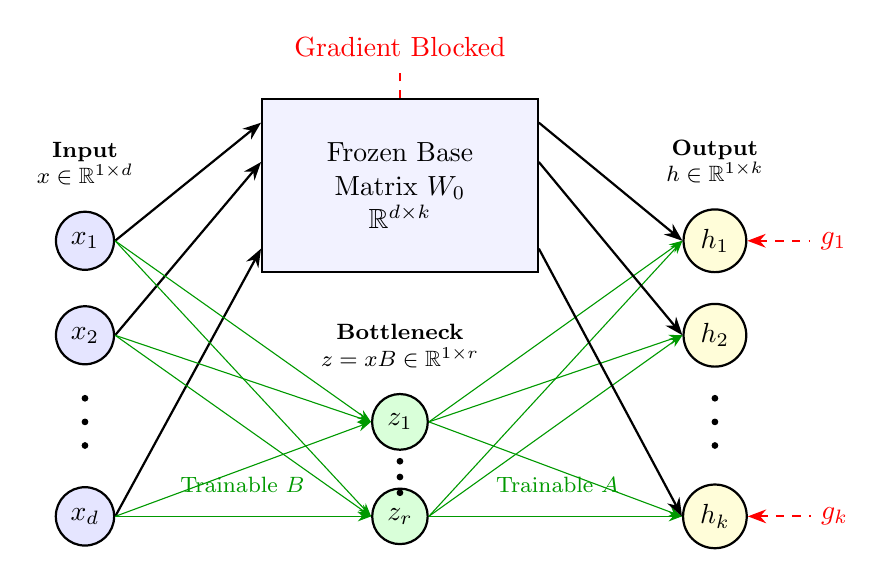
\begin{tikzpicture}[
  neuron/.style={circle, draw, minimum size=0.6cm, fill=blue!10, thick},
  bottleneck/.style={circle, draw, minimum size=0.6cm, fill=green!15, thick},
  out_neuron/.style={circle, draw, minimum size=0.6cm, fill=yellow!15, thick},
  arrow/.style={-Stealth, thick},
  grad_arrow/.style={Stealth-, red, dashed, thick},
  layer_label/.style={align=center, font=\footnotesize\bfseries}
]

  % Input Layer Neurons
  \node[neuron] (x1) at (0, 2.5) {$x_1$};
  \node[neuron] (x2) at (0, 1.3) {$x_2$};
  \node[coordinate] (xdots) at (0, 0) {};
  \node[neuron] (xd) at (0, -1.0) {$x_d$};
  \draw[fill] (0,0.5) circle (1pt);
  \draw[fill] (0,0.2) circle (1pt);
  \draw[fill] (0,-0.1) circle (1pt);
  \node[layer_label, above=0.2cm of x1] {Input \\ $x \in \mathbb{R}^{1 \times d}$};

  % Frozen Weights Box (Placed higher up to avoid crossing paths)
  \node[draw, rectangle, minimum width=3.5cm, minimum height=2.2cm, fill=blue!5, thick, align=center] (W0) at (4.0, 3.2) {Frozen Base \\ Matrix $W_0$ \\ $\mathbb{R}^{d \times k}$};

  % Bottleneck Layer Neurons (Rank r)
  \node[bottleneck] (z1) at (4.0, 0.2) {$z_1$};
  \node[coordinate] (zdots) at (4.0, -0.3) {};
  \node[bottleneck] (zr) at (4.0, -1.0) {$z_r$};
  \draw[fill] (4.0,-0.3) circle (1pt);
  \draw[fill] (4.0,-0.5) circle (1pt);
  \draw[fill] (4.0,-0.7) circle (1pt);
  \node[layer_label, above=0.2cm of z1] {Bottleneck \\ $z = xB \in \mathbb{R}^{1 \times r}$};

  % Output Layer Neurons
  \node[out_neuron] (h1) at (8.0, 2.5) {$h_1$};
  \node[out_neuron] (h2) at (8.0, 1.3) {$h_2$};
  \node[coordinate] (hdots) at (8.0, 0) {};
  \node[out_neuron] (hk) at (8.0, -1.0) {$h_k$};
  \draw[fill] (8.0,0.5) circle (1pt);
  \draw[fill] (8.0,0.2) circle (1pt);
  \draw[fill] (8.0,-0.1) circle (1pt);
  \node[layer_label, above=0.2cm of h1] {Output \\ $h \in \mathbb{R}^{1 \times k}$};

  % Connections: Input -> W0
  \draw[arrow] (x1.east) -- ($(W0.west)+(0,0.8)$);
  \draw[arrow] (x2.east) -- ($(W0.west)+(0,0.3)$);
  \draw[arrow] (xd.east) -- ($(W0.west)+(0,-0.8)$);

  % Connections: Input -> Bottleneck via B (Trainable)
  \foreach \i in {x1, x2, xd} {
    \foreach \j in {z1, zr} {
      \draw[arrow, green!60!black, thin] (\i.east) -- (\j.west);
    }
  }
  \node[green!60!black, font=\footnotesize] at (2.0, -0.6) {Trainable $B$};

  % Connections: Bottleneck -> Output via A (Trainable)
  \foreach \i in {z1, zr} {
    \foreach \j in {h1, h2, hk} {
      \draw[arrow, green!60!black, thin] (\i.east) -- (\j.west);
    }
  }
  \node[green!60!black, font=\footnotesize] at (6.0, -0.6) {Trainable $A$};

  % Connections: W0 -> Output
  \draw[arrow] ($(W0.east)+(0,0.8)$) -- (h1.west);
  \draw[arrow] ($(W0.east)+(0,0.3)$) -- (h2.west);
  \draw[arrow] ($(W0.east)+(0,-0.8)$) -- (hk.west);

  % Backward pass annotations
  \draw[grad_arrow] (h1.east) -- ++(0.8,0) node[right, red] {$g_1$};
  \draw[grad_arrow] (hk.east) -- ++(0.8,0) node[right, red] {$g_k$};

  \draw[red, dashed, thick] (W0.north) -- ++(0,0.4) node[above, red] {Gradient Blocked};

\end{tikzpicture}
\caption{Neuron-level forward path (solid arrows) and backward gradient routing (dashed red arrows).}
\end{figure}

\newpage
\section{Functional Pipelines: Before State, After State, and Flow Control}

We present the complete code implementation, before and after states, and dedicated transformation flow diagrams for each helper function.

\subsection{Model and Tokenizer Loader: \texttt{initialize\_base\_model}}

\subsubsection{Functional Code Implementation}
The initializer handles loading vocabulary parameters and floating-point representations of the model weights from the local cache directory. Memory bounds are defined based on precision casting.

\begin{lstlisting}[language=Python]
from transformers import AutoModelForCausalLM, AutoTokenizer
import torch

def initialize_base_model(model_id="Qwen/Qwen2.5-0.5B-Instruct"):
    tokenizer = AutoTokenizer.from_pretrained(model_id, trust_remote_code=True)
    tokenizer.pad_token = tokenizer.eos_token

    # Setup hardware parameters automatically based on GPU compatibility
    torch_dtype = torch.bfloat16 if torch.cuda.is_bf16_supported() else torch.float16
    device_map = "auto" if torch.cuda.is_available() else "cpu"

    model = AutoModelForCausalLM.from_pretrained(
        model_id,
        torch_dtype=torch_dtype,
        device_map=device_map,
        trust_remote_code=True
    )
    return model, tokenizer
\end{lstlisting}

\subsubsection{Parameter States Table}
\begin{table}[h]
\centering
\begin{tabular}{lll}
\toprule
\textbf{Property} & \textbf{Before State} & \textbf{After State} \\
\midrule
RAM Allocation & $0$ MB & $\approx 1024$ MB \\
Loaded Variables & None & Model (CausalLM) + Tokenizer \\
Weight Matrix Shape $W_0$ & Unloaded & $\mathbb{R}^{896 \times 896}$ \\
Embedding Matrix Shape $W_{\text{embed}}$ & Unloaded & $\mathbb{R}^{151936 \times 896}$ \\
Grad Requirements & None & $\text{requires\_grad} = \text{True}$ \\
\bottomrule
\end{tabular}
\caption{State properties and shapes for model initialization.}
\end{table}

\newpage
\subsubsection{Logical Transformation Flow (\texttt{initialize\_base\_model})}
This diagram visualizes weight file retrieval from disk storage, decompression/casting in the loading stream, and allocations into system memory.

\begin{figure}[h]
\centering
\begin{center}
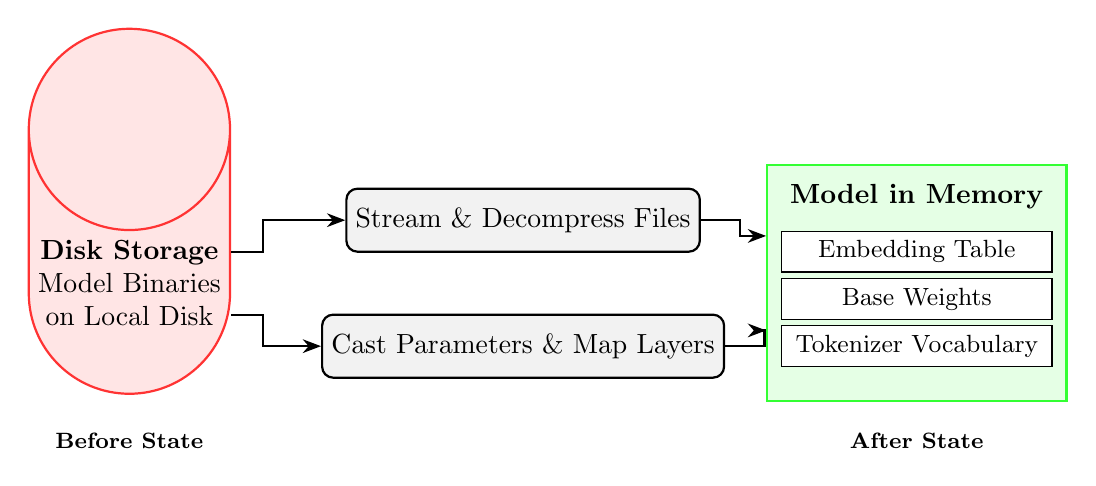
\begin{tikzpicture}[
  arrow/.style={-Stealth, thick},
  cylinder_box/.style={cylinder, draw, shape border rotate=90, minimum width=2.0cm, minimum height=2.2cm, fill=red!10, draw=red!80, thick, align=center},
  ram_box/.style={draw, rectangle, minimum width=3.8cm, minimum height=3.0cm, fill=green!10, draw=green!80, thick, align=center},
  pipe_box/.style={draw, rounded corners, minimum width=3.5cm, minimum height=0.8cm, fill=gray!10, thick, align=center}
]

  % BEFORE: Disk Storage Icon
  \node (disk) [cylinder_box] at (-5.0, 0) {\textbf{Disk Storage} \\ Model Binaries \\ on Local Disk};
  \node[align=center, font=\footnotesize] at (-5.0, -2.0) {\textbf{Before State}};

  % PIPELINE: Data Transformations
  \node (cast) [pipe_box] at (0, 0.8) {Stream \& Decompress Files};
  \node (map) [pipe_box] at (0, -0.8) {Cast Parameters \& Map Layers};

  % AFTER: RAM Blocks
  \node (ram) [ram_box] at (5.0, 0) {};
  \node at (5.0, 1.1) {\textbf{Model in Memory}};
  \node[draw, fill=white, font=\small, text width=3.2cm, align=center] at (5.0, 0.4) {Embedding Table};
  \node[draw, fill=white, font=\small, text width=3.2cm, align=center] at (5.0, -0.2) {Base Weights};
  \node[draw, fill=white, font=\small, text width=3.2cm, align=center] at (5.0, -0.8) {Tokenizer Vocabulary};
  \node[align=center, font=\footnotesize] at (5.0, -2.0) {\textbf{After State}};

  % Connections
  \draw[arrow] ($(disk.east)+(0,0.4)$) -- ++(0.4,0) |- (cast.west);
  \draw[arrow] ($(disk.east)-(0,0.4)$) -- ++(0.4,0) |- (map.west);
  \draw[arrow] (cast.east) -- ++(0.5,0) |- ($(ram.west)+(0,0.6)$);
  \draw[arrow] (map.east) -- ++(0.5,0) |- ($(ram.west)+(0,-0.6)$);

\end{tikzpicture}
\end{center}
\caption{System load transformation mapping disk-based weights to RAM tensors.}
\end{figure}

\newpage
\subsection{PEFT Wrapper Layer Adapter: \texttt{apply\_lora\_adapters}}

\subsubsection{Functional Code Implementation}
Adapter parameters are structured to map dimensions from activation scale $d$ to constraint bottleneck rank $r$. Layer weights parameters are wrapped to reroute backpropagation pipelines.

\begin{lstlisting}[language=Python]
from peft import LoraConfig, get_peft_model, TaskType

def apply_lora_adapters(model, rank=8, alpha=16):
    peft_config = LoraConfig(
        task_type=TaskType.CAUSAL_LM,
        r=rank,
        lora_alpha=alpha,
        lora_dropout=0.05,
        target_modules=["q_proj", "k_proj", "v_proj", "o_proj", "gate_proj", "up_proj", "down_proj"],
        bias="none"
    )
    # Wraps the model and freezes base weight parameters automatically
    model = get_peft_model(model, peft_config)
    return model
\end{lstlisting}

\subsubsection{Parameter States Table}
\begin{table}[h]
\centering
\begin{tabular}{lll}
\toprule
\textbf{Property} & \textbf{Before State} & \textbf{After State} \\
\midrule
Layer Wrapping & Plain CausalLM Linear & PEFT Wrapped Module \\
Base Weights $W_0$ Grads & $\text{requires\_grad} = \text{True}$ & $\text{requires\_grad} = \text{False}$ (Frozen) \\
Trainable Parameters & $\approx 500$ Million & $\approx 6.2$ Million (LoRA matrices) \\
LoRA Matrix $B$ Shape & Does not exist & $\mathbb{R}^{896 \times 8}$ (Initialized to $0$) \\
LoRA Matrix $A$ Shape & Does not exist & $\mathbb{R}^{8 \times 896}$ (Initialized to Gaussian) \\
\bottomrule
\end{tabular}
\caption{State details before and after adapter injection.}
\end{table}

\newpage
\subsubsection{Logical Transformation Flow (\texttt{apply\_lora\_adapters})}
This diagram maps the structural change of a linear mapping, shifting from a single active matrix to a frozen base weight matrix bypassed by trainable low-rank path networks.

\begin{figure}[h]
\centering
\begin{center}
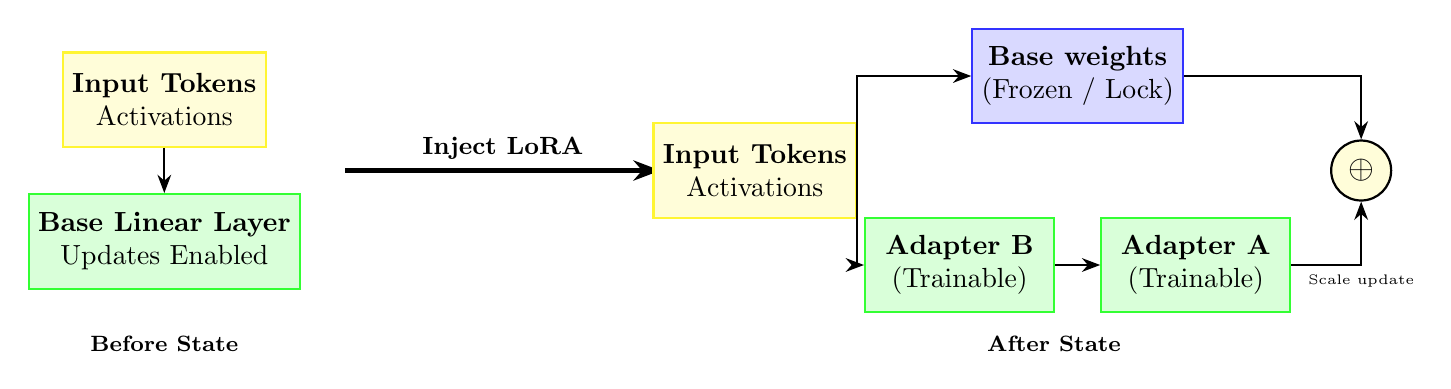
\begin{tikzpicture}[
  arrow/.style={-Stealth, thick},
  block/.style={draw, rectangle, minimum width=2.4cm, minimum height=1.2cm, thick, align=center},
  frozen_block/.style={block, fill=blue!15, draw=blue!80},
  trainable_block/.style={block, fill=green!15, draw=green!80},
  input_block/.style={block, fill=yellow!15, draw=yellow!80}
]

  % BEFORE: CausalLM Native Linear Layer
  \node (in_before) [input_block] at (-4.5, 1.8) {\textbf{Input Tokens} \\ Activations};
  \node (w0_before) [trainable_block] at (-4.5, 0.0) {\textbf{Base Linear Layer} \\ Updates Enabled};
  \draw[arrow] (in_before.south) -- (w0_before.north);
  \node[align=center, font=\footnotesize] at (-4.5, -1.3) {\textbf{Before State}};

  % TRANSFORMATION PIPELINE MIDDLE
  \draw[arrow, line width=1.5pt] (-2.2, 0.9) -- node[above, font=\small\bfseries] {Inject LoRA} (1.8, 0.9);

  % AFTER: LoRA Wrapped Pathway
  \node (in_after) [input_block] at (3.0, 0.9) {\textbf{Input Tokens} \\ Activations};
  \node (w0_after) [frozen_block] at (7.1, 2.1) {\textbf{Base weights} \\ (Frozen / Lock)};
  
  \node (b_after) [trainable_block] at (5.6, -0.3) {\textbf{Adapter B} \\ (Trainable)};
  \node (a_after) [trainable_block] at (8.6, -0.3) {\textbf{Adapter A} \\ (Trainable)};
  \node (sum) [circle, draw, thick, minimum size=0.6cm, fill=yellow!15] at (10.7, 0.9) {\large \(\oplus\)};

  \draw[arrow] (in_after.east) |- (w0_after.west);
  \draw[arrow] (in_after.east) |- (b_after.west);
  \draw[arrow] (b_after.east) -- (a_after.west);
  \draw[arrow] (w0_after.east) -| (sum.north);
  \draw[arrow] (a_after.east) -| (sum.south) node[midway, below, font=\tiny] {Scale update};
  \node[align=center, font=\footnotesize] at (6.8, -1.3) {\textbf{After State}};

\end{tikzpicture}
\end{center}
\caption{Parameter transformation flow mapping adapter logic injection.}
\end{figure}

\newpage
\subsection{Tokenization and Label Masking: \texttt{tokenize\_and\_mask\_labels}}

\subsubsection{Functional Code Implementation}
Preprocesses raw template sequences, formatting system instructions and isolating debugger output strings for loss computation mapping.

\begin{lstlisting}[language=Python]
def tokenize_and_mask_labels(examples, tokenizer):
    prompts = [f"<|im_start|>system\nYou are a formatting engine for pylow. Output ASCII layout layout correctly.<|im_end|>\n<|im_start|>user\n{inp}<|im_end|>\n<|im_start|>assistant\n" for inp in examples["input"]]
    targets = [f"{out}<|im_end|>" for out in examples["output"]]
    
    inputs = tokenizer(prompts, add_special_tokens=False)
    labels = tokenizer(targets, add_special_tokens=False)
    
    input_ids = []
    label_ids = []
    for i in range(len(prompts)):
        # Concatenate prompt inputs and output targets
        input_ids.append(inputs["input_ids"][i] + labels["input_ids"][i])
        # Mask out system prompt sequence with -100
        label_ids.append([-100] * len(inputs["input_ids"][i]) + labels["input_ids"][i])
        
    return {"input_ids": input_ids, "labels": label_ids}
\end{lstlisting}

\subsubsection{Parameter States Table}
\begin{table}[h]
\centering
\begin{tabular}{lll}
\toprule
\textbf{Property} & \textbf{Before State} & \textbf{After State} \\
\midrule
Format Type & Raw Python Strings & Integer Tensors \\
Input IDs Shape & $1$ (Scalar String) & $\mathbb{Z}^{\text{seq\_len}}$ \\
Label IDs Shape & $1$ (Scalar String) & $\mathbb{Z}^{\text{seq\_len}}$ \\
Prompt Labels Value & Raw string representation & Masked out with $-100$ \\
Response Labels Value & Raw string representation & Int token identifiers preserved \\
\bottomrule
\end{tabular}
\caption{Data structures before and after tokenization.}
\end{table}

\newpage
\subsubsection{Logical Transformation Flow (\texttt{tokenize\_and\_mask\_labels})}
This visual mapping details how text strings translate to aligned vocabulary integer indices, showing exactly how prompt loss calculation parameters are masked out.

\begin{figure}[h]
\centering
\begin{center}
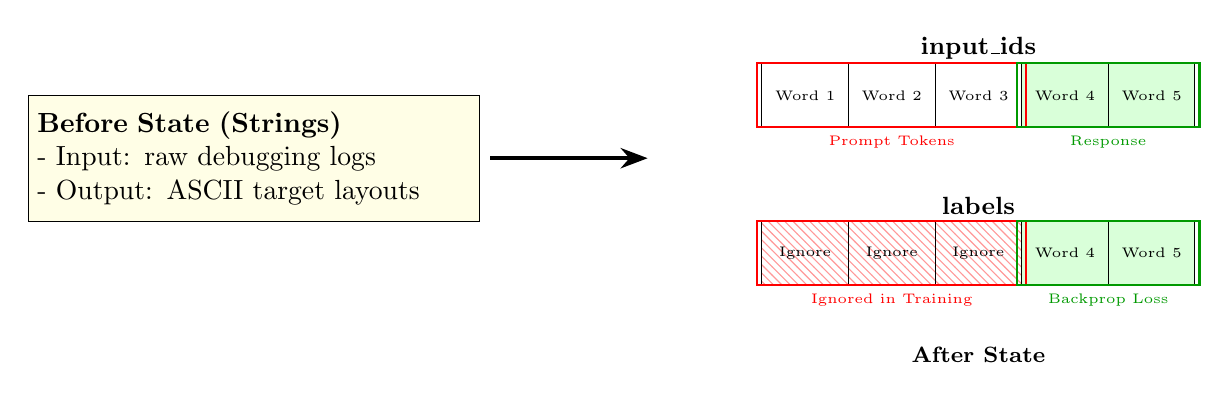
\begin{tikzpicture}[
  arrow/.style={-Stealth, thick},
  cell/.style={draw, rectangle, minimum width=1.1cm, minimum height=0.8cm, align=center, fill=white, font=\tiny},
  masked_cell/.style={cell, pattern=north west lines, pattern color=red!40},
  lbl/.style={font=\small\bfseries, align=center}
]

  % BEFORE: String JSON Inputs
  \node[draw, fill=yellow!10, text width=5.5cm, minimum height=1.6cm, align=left] (before) at (-5.0, 0) {
    \textbf{Before State (Strings)} \\
    - Input: raw debugging logs \\
    - Output: ASCII target layouts
  };

  % PIPELINE
  \draw[arrow, line width=1.5pt] (-2.0, 0) -- (0, 0);

  % AFTER: Aligned Array Grids
  % Input IDs Row
  \node[lbl] at (4.2, 1.4) {input\_ids};
  \node[cell] (i1) at (2.0, 0.8) {Word 1};
  \node[cell] (i2) at (3.1, 0.8) {Word 2};
  \node[cell] (i3) at (4.2, 0.8) {Word 3};
  \node[cell, fill=green!15] (i4) at (5.3, 0.8) {Word 4};
  \node[cell, fill=green!15] (i5) at (6.4, 0.8) {Word 5};
  
  \draw[thick, red] ($(i1.north west)-(0.05,0)$) rectangle ($(i3.south east)+(0.05,0)$);
  \node[red, font=\tiny] at (3.1, 0.2) {Prompt Tokens};
  
  \draw[thick, green!60!black] ($(i4.north west)-(0.05,0)$) rectangle ($(i5.south east)+(0.05,0)$);
  \node[green!60!black, font=\tiny] at (5.85, 0.2) {Response};

  % Labels IDs Row
  \node[lbl] at (4.2, -0.6) {labels};
  \node[masked_cell] (l1) at (2.0, -1.2) {Ignore};
  \node[masked_cell] (l2) at (3.1, -1.2) {Ignore};
  \node[masked_cell] (l3) at (4.2, -1.2) {Ignore};
  \node[cell, fill=green!15] (l4) at (5.3, -1.2) {Word 4};
  \node[cell, fill=green!15] (l5) at (6.4, -1.2) {Word 5};
  
  \draw[thick, red] ($(l1.north west)-(0.05,0)$) rectangle ($(l3.south east)+(0.05,0)$);
  \node[red, font=\tiny] at (3.1, -1.8) {Ignored in Training};
  
  \draw[thick, green!60!black] ($(l4.north west)-(0.05,0)$) rectangle ($(l5.south east)+(0.05,0)$);
  \node[green!60!black, font=\tiny] at (5.85, -1.8) {Backprop Loss};

  \node[align=center, font=\footnotesize] at (4.2, -2.5) {\textbf{After State}};

\end{tikzpicture}
\end{center}
\caption{Parameter transformation flow mapping string sequences to masked label tokens.}
\end{figure}

\newpage
\subsection{Training Execution Loop: \texttt{execute\_training\_loop}}

\subsubsection{Functional Code Implementation}
The training execution block establishes micro-batch iterations, gradient scaling accumulation limits, and logs parameter updates to disk files.

\begin{lstlisting}[language=Python]
from transformers import TrainingArguments, Trainer, DataCollatorForSeq2Seq

def execute_training_loop(model, tokenizer, tokenized_dataset, output_path):
    training_args = TrainingArguments(
        output_dir=output_path,
        per_device_train_batch_size=2,
        gradient_accumulation_steps=4,
        learning_rate=2e-4,
        logging_steps=10,
        num_train_epochs=3,
        save_strategy="epoch",
        evaluation_strategy="no",
        fp16=False,
        bf16=False,
        optim="adamw_torch"
    )
    
    trainer = Trainer(
        model=model,
        args=training_args,
        train_dataset=tokenized_dataset,
        data_collator=DataCollatorForSeq2Seq(tokenizer=tokenizer, pad_to_multiple_of=8, return_tensors="pt", padding=True)
    )
    trainer.train()
    model.save_pretrained(f"{output_path}/adapter")
\end{lstlisting}

\subsubsection{Parameter States Table}
\begin{table}[h]
\centering
\begin{tabular}{lll}
\toprule
\textbf{Property} & \textbf{Before State} & \textbf{After State} \\
\midrule
Adapter Parameters & $A \sim \mathcal{N}(0, \sigma^2)$, $B = 0$ & Optimized weights $A^*, B^*$ \\
Causal LM Loss & $\mathcal{L} \approx 10.0$ & $\mathcal{L} < 0.1$ \\
Active Memory Footprint & $1024$ MB (weights) & $1024$ MB + Optimizer states \\
Checkpoints & Empty directory & Adapter weights saved on disk \\
\bottomrule
\end{tabular}
\caption{Parameter states and loss during the training phase.}
\end{table}

\newpage
\subsubsection{Logical Transformation Flow (\texttt{execute\_training\_loop})}
The diagram below details the forward-backward optimization loop that updates the trainable adapter parameters.

\begin{figure}[h]
\centering
\begin{center}
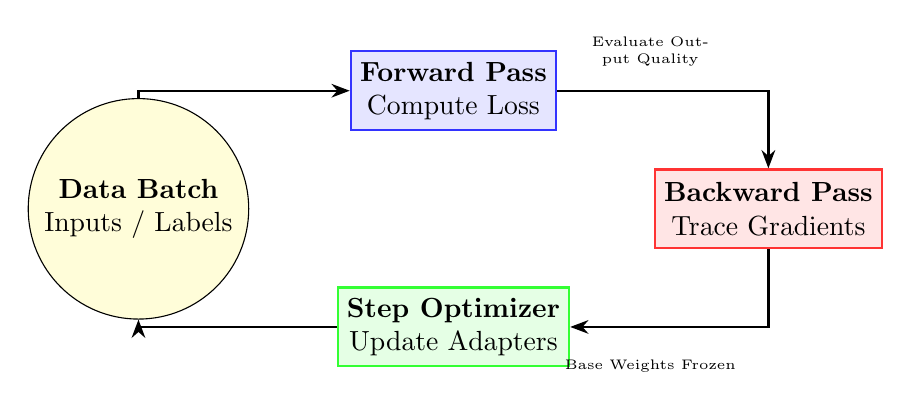
\begin{tikzpicture}[
  arrow/.style={-Stealth, thick},
  block/.style={draw, rectangle, minimum width=2.5cm, minimum height=1.0cm, thick, align=center},
  fwd_block/.style={block, fill=blue!10, draw=blue!80},
  bwd_block/.style={block, fill=red!10, draw=red!80},
  opt_block/.style={block, fill=green!10, draw=green!80}
]

  % Core optimization loop visualizer
  \node (batch) [draw, circle, fill=yellow!15, minimum size=1.8cm, align=center] at (-4.0, 0) {\textbf{Data Batch} \\ Inputs / Labels};
  \node (fwd) [fwd_block] at (0, 1.5) {\textbf{Forward Pass} \\ Compute Loss};
  \node (bwd) [bwd_block] at (4.0, 0) {\textbf{Backward Pass} \\ Trace Gradients};
  \node (opt) [opt_block] at (0, -1.5) {\textbf{Step Optimizer} \\ Update Adapters};

  % Circular Arrows
  \draw[arrow] (batch.north) |- (fwd.west);
  \draw[arrow] (fwd.east) -| (bwd.north);
  \draw[arrow] (bwd.south) |- (opt.east);
  \draw[arrow] (opt.west) -| (batch.south);

  % Annotations (Adjusted coordinates to avoid overlapping boxes)
  \node[font=\tiny, text width=2.2cm, align=center] at (2.5, 2.0) {Evaluate Output Quality};
  \node[font=\tiny, text width=2.2cm, align=center] at (2.5, -2.0) {Base Weights Frozen};

\end{tikzpicture}
\end{center}
\caption{Circular flow mapping of the training step execution loop.}
\end{figure}

\newpage
\subsection{Zero-Overhead Deployment Merge: \texttt{merge\_adapters\_for\_deployment}}

\subsubsection{Functional Code Implementation}
Resolves model output path speed penalties by collapsing trainable parameters back into fixed weights.

\begin{lstlisting}[language=Python]
from peft import PeftModel

def merge_adapters_for_deployment(base_model_id, adapter_path, merged_output_path):
    base_model = AutoModelForCausalLM.from_pretrained(
        base_model_id,
        torch_dtype=torch.float16,
        device_map="cpu"
    )
    # Attach adapter parameters
    peft_model = PeftModel.from_pretrained(base_model, adapter_path)
    
    # Merge BA into W_0 and unload PEFT packaging
    merged_model = peft_model.merge_and_unload()
    
    # Serialize to disk
    merged_model.save_pretrained(merged_output_path)
    print("Merged weights saved successfully!")
\end{lstlisting}

\subsubsection{Parameter States Table}
\begin{table}[h]
\centering
\begin{tabular}{lll}
\toprule
\textbf{Property} & \textbf{Before State} & \textbf{After State} \\
\midrule
PEFT Wrapping & Wrapper active in memory & Removed \\
Active Parameter Sets & $\{W_0, B, A\}$ (Three matrices) & $\{W_{\text{deploy}}\}$ (Single matrix) \\
Layer Output Comp. & $h = xW_0 + \frac{\alpha}{r}xBA$ & $h = xW_{\text{deploy}}$ \\
Inference Overhead & Extra matrix multiplication & Zero extra latency \\
Weights File shape & Base + Adapter binaries & Unified model weights binary \\
\bottomrule
\end{tabular}
\caption{Parameter representations during adapter merging.}
\end{table}

\newpage
\subsubsection{Logical Transformation Flow (\texttt{merge\_adapters\_for\_deployment})}
This diagram maps parameter addition, merging parallel layers into a single weight tensor.

\begin{figure}[h]
\centering
\begin{center}
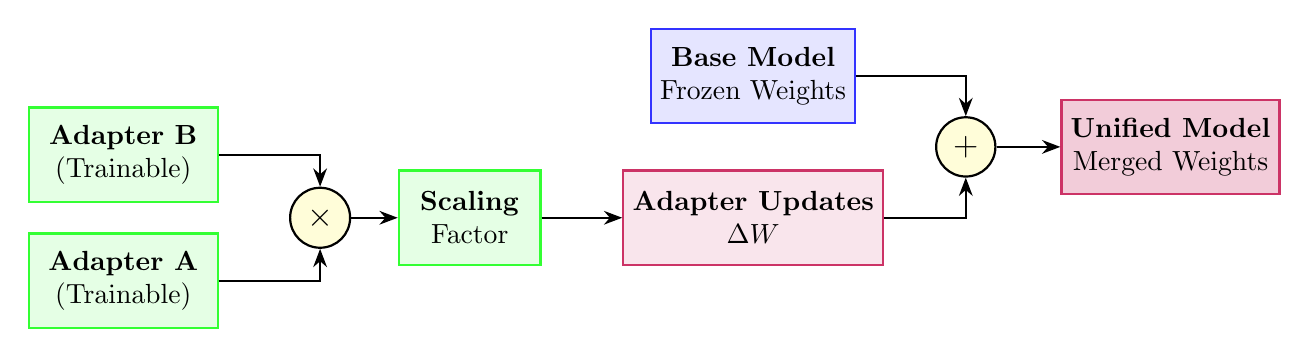
\begin{tikzpicture}[
  arrow/.style={-Stealth, thick},
  matrix_box/.style={draw, rectangle, fill=blue!10, draw=blue!80, thick, minimum width=2.4cm, minimum height=1.2cm, align=center},
  adapter_box/.style={draw, rectangle, fill=green!10, draw=green!80, thick, minimum width=2.4cm, minimum height=1.2cm, align=center},
  merged_box/.style={draw, rectangle, fill=purple!10, draw=purple!80, thick, minimum width=2.4cm, minimum height=1.2cm, align=center}
]

  % BEFORE: Disjoint base + adapter weights (No overlaps, coordinates explicitly spaced)
  \node (B) [adapter_box] at (-7.5, 0.8) {\textbf{Adapter B} \\ (Trainable)};
  \node (A) [adapter_box] at (-7.5, -0.8) {\textbf{Adapter A} \\ (Trainable)};
  
  \node (times) [circle, draw, thick, fill=yellow!15, minimum size=0.6cm] at (-5.0, 0.0) {\large $\times$};
  \node (scale) [adapter_box, minimum width=1.8cm] at (-3.1, 0.0) {\textbf{Scaling} \\ Factor};
  \node (delta_w) [merged_box] at (0.5, 0.0) {\textbf{Adapter Updates} \\ \(\Delta W\)};
  
  \node (W0) [matrix_box] at (0.5, 1.8) {\textbf{Base Model} \\ Frozen Weights};
  
  \node (plus) [circle, draw, thick, fill=yellow!15, minimum size=0.6cm] at (3.2, 0.9) {\large $+$};
  \node (w_deploy) [merged_box, fill=purple!20] at (5.8, 0.9) {\textbf{Unified Model} \\ Merged Weights};

  % Connections
  \draw[arrow] (B.east) -| (times.north);
  \draw[arrow] (A.east) -| (times.south);
  \draw[arrow] (times.east) -- (scale.west);
  \draw[arrow] (scale.east) -- (delta_w.west);
  \draw[arrow] (W0.east) -| (plus.north);
  \draw[arrow] (delta_w.east) -| (plus.south);
  \draw[arrow] (plus.east) -- (w_deploy.west);

\end{tikzpicture}
\end{center}
\caption{Consolidation flow of multiple weights paths into a single deployment matrix.}
\end{figure}

\end{document}
